\documentclass[onecolumn,10pt]{IEEEtran}

\usepackage{graphicx}
\usepackage{siunitx}
\usepackage{amsmath,amsfonts,amssymb}
%\usepackage{marginnote} % for editorial use
\usepackage{sidenotes} % for editorial use

\newcommand{\myroot}{../}
\newcommand{\Later}{\textbf{Later.}}
\newcommand{\Calypteanna}{\emph{Calypte anna}}
\newcommand{\MATLAB}{MATLAB}


\title{Autonomous trajectory planning to copy bird-like maneuvers}
\author{E.~Marcello and D.~Evangelista\thanks{Authors are with the United States Naval Academy, Department of Weapons, Robotics, and Control Engineering}}
\date{today}

\begin{document}
\maketitle

\begin{abstract}
Abstract here. \Later
\end{abstract}

\begin{IEEEkeywords}
capstone, robotics, controls
\end{IEEEkeywords}

\section{Background and motivation}
\IEEEPARstart{T}{he origin of this type of research} stems from the desire to solve engineering problems by studying the way that biological organisms overcome a similar problem. As an example, the monocopter is a device that is able to fly using the same aerodynamic principles of the “helicopter” maple seeds. Maple seeds are able to slow their decent to the ground using a particular weight distribution and wing structure to facilitate autorotation. This allows them to be carried by the wind instead of simply falling straight down to the base of the tree, which can be advantageous for the growth of the new maple saplings. Researchers in \cite{who2019maple} developed a monocopter based off of this concept, and were able to develop a control algorithm that allowed them to control the direction of the flying UAV. This design may never have been created if it weren’t for the careful study of the maple seeds and their curious aerodynamic properties. 

On the other hand, sometimes a robot is created for the sake of learning more about a specific type of biological behavior. In \cite{feltman2014creepy}, the strange movement behavior seen by the sidewinder rattlesnake is studied by creating a robot to imitate it. Sidewinders get their name from the way that they seem to travel sideways in a twisting-lurching type fashion across the hot desert sand. The robot was developed like a snake, and was programmed to copy as closely as possible the movement\sidenote{test} of the sidewinder. The initial test had success on level ground, but no such luck on steeper slopes. It wasn’t until then that the discovery was made that the sidewinder used two independent wavelike motions to move instead of just a single wave. Once this was implemented to the design, the robot was able to navigate just like the sidewinder, and a new form of ground travel was made attainable by robotic machines. This discovery has applications of movement over a variety of different terrain that a typical wheeled robot would have significant trouble with.

In the case of my research, I will be attempting to enhance a quadrotor’s maneuverability by studying the flight patterns and maneuvers of different types of hummingbirds, specifically Anna’s Hummingbirds (\Calypteanna). With the huge influx of research in quadrotor control, it has become apparent, especially in \cite{mellinger2011minimum, greiff2017modelling}, that the next step for the development of autonomous aerial vehicles is extreme maneuverability. Air platforms are becoming increasingly more autonomous, which begs the question, how far can autonomy really take UAVs? From level flight, to obstacle avoidance, path planning and trajectory matching, autonomous vehicles are beginning to show promise of greatly surpassing any human operator in safety and performance. My research seeks to develop an autonomous solution of executing a highly stressful maneuver, specifically to match the flight maneuvers performed by Anna’s Hummingbirds. 

I chose Anna’s Hummingbirds to be modeled after for my research because of both their impressive dive patterns, and also the relative abundance of data collected on these dives. In \cite{larimer1995accelerational}, the researchers describe the hummingbird dives to have accelerations of up to \SIrange{7}{10}{g}, with the hummingbirds reaching a maximum velocity of approximately \SI{20}{\meter\per\second} at the start of the pull-out phase of their dive. Such numbers are astronomically large for an organism with a mass less than \SI{5}{\gram}; and could cause g-induced loss of consciousness (GLOC) in a human pilot without a g-suit. As a result, the maneuver must expend a large amount of energy to complete, and it is likely extremely difficult for a quadrotor to imitate. I intend to discover how feasible the dive maneuvers actually are for quadrotors, and explore their operational limits in this respect. 

The applications of this research are twofold: it will both help in developing a greater understanding of the physical limitations of extreme maneuverability on quadrotors, and it will also provide a greater idea of the effects of these dive maneuvers on the hummingbirds. The ability to automate the hummingbird dive maneuvers means that other forms of extreme maneuvers can also be autonomously executed. As a result, the mission set for autonomous UAVs and MAVs is greatly increased, as they will have an increased maneuvering ability. If combined with enhanced sensing abilities, autonomous MAVs would be able to navigate through obstacle-heavy environments with greater speed and ease. In addition, evasive maneuvers could aid many UAVs from being downed by a net, or other harmful projectiles. 

In addition to this, a successful maneuver could be used to probe live hummingbirds to see how they react. Since these dive maneuvers are used in male courtship ceremonies, if a quadrotor were to execute this dive in front of an unsuspecting female bird, could the quadrotor generate a favorable response from her? If so, it may be possible to tweak the dive pattern and discover what aspect of the dive the females find most appealing, whether it is speed, sound, dive shape, or some other aspect that prior researchers have overlooked. The ability to successfully replicate these maneuvers could open up an entirely new biological study concerning hummingbird courtship displays, and bring to light new information about these biological feats of nature.

\section{Problem statement}
The aim of my research is to replicate the display dives of Anna’s Hummingbirds (\Calypteanna) with an autonomous quadrotor platform. My project assumes the following are provided: a quadrotor platform, a flight controller, and a method of obtaining three-dimensional (3D) position data of the quadrotor in test flights. I also assume that all position vs. time data related to the hummingbird dive trajectories are given, and that each trajectory can be approximated as a fourth degree polynomial function in a fixed 3D right handed coordinate frame. Given a desired hummingbird flight trajectory, depicted in Figure~\ref{fig-problem-statement-1}a, my quadrotor will autonomously generate and execute the control inputs required to successfully complete the maneuver. 

A successful maneuver is defined as a root mean square error calculation of less than \SI{5}{\percent} between the time-scaled hummingbird trajectory and the quadrotor trajectory, where each trajectory is defined as a matrix array of positions in the $x$, $y$, $z$ right handed coordinate frame with a given sample period, $\delta t$. The hummingbird trajectory will be scaled by a constant factor in time to allow for the physical limitations of the quadrotor—e.g. the quadrotor may only have to travel the desired trajectory at half the speed of the hummingbird to still achieve a successful maneuver. This is a necessary adaptation due to the impressive speed and acceleration capabilities of the Anna’s hummingbirds relative to their size \cite{clark2009courtship}. The ideal result is to fly the hummingbird trajectory at the same speed as the hummingbird, but this may prove to be impossible due to the physical constraints of the quadrotor.
\begin{figure}[h]
\begin{center}
\includegraphics[height=1.88in]{\myroot/figures/problem-statement-1a.png}%
\includegraphics[height=1.88in]{\myroot/figures/problem-statement-1b.png}
\end{center}
\caption{(a) The five stages of an Anna’s Hummingbird dive maneuver, from \cite{clark2009courtship}. (b) A quadrotor using path planning to fly through a thrown hoop, from \cite{mellinger2011minimum}.}
\label{fig-problem-statement-1}
\end{figure}

As a stretch goal, I will also analyze and replicate a variety of different types of hummingbird dives and maneuvers, to include evasive aerial maneuvers. Success will be determined in the same fashion as described above.

\section{Literature review}
The inspiration of this project proposal has its roots in the high maneuverability seen by hummingbirds. As such, it was essential to be able to gather data on hummingbird trajectories in order to study their feasibility of being replicated by a quadrotor. There have been many bio researchers that have delved into the study of hummingbirds, however I will mainly discuss the works \cite{clark2009courtship} and \cite{cheng2016flight}. The work in \cite{cheng2016flight} determined the trajectory and body kinematics of four different hummingbird species in an evasive maneuver. This was done by startling the birds while they were hovering, and observing their movements with 3 high definition cameras to provide a 3D position. Water-soluble white paint was used to make dot markings on the hummingbird’s body to help model the wing and head positions for each trial. The data they acquired in their experiments includes many more details than I will need to use, however they provide data on the hummingbird’s velocity and trajectories for several trials which I can use to help develop my quadrotor trajectories. I will even use a similar tracking method as \cite{cheng2016flight}, they and I will both be using optical data to obtain a position fix. With regard to the type of maneuver that these birds are required to perform, it aligns well with the type of experimentation that I aim to work with. Evasive maneuvers are certainly a type of extreme maneuver, and these patterns may prove to be something that I wish to try on my quadrotor. Evasive maneuvers can be useful for quadrotors if they are in threat of being netted, and if I am able to copy the hummingbird’s trajectory, further analysis and testing may prove that this type of trajectory provides a maneuvering or sensing advantage to the quadrotor in evasive flight.

The work in \cite{clark2009courtship} has also obtained very accurate data on hummingbird flight trajectories. This work specifically pertains to the study of the Anna’s hummingbird’s courtship dives in order to study extreme locomotor performance in animals. This was done using several cameras of varying resolution and frame rate to record the male hummingbird’s dives. The video results were digitized using Peak Motus 8, and analyzed using mathematical relationships to determine the accelerations, velocities, flight paths, wing/tail movements of, and sounds produced by the hummingbirds in their dives. Again, this is more detailed data than I will need for trajectory replication on my quadrotor. This paper gives an insight into what exactly I will be trying to achieve through the extreme maneuverability of my quadrotor. Since this type of maneuver is estimated to cause a lot of strain on the hummingbird, it is likely to also cause a lot of strain on a quadrotor. Through simulation and proof of concept demonstration, I will be able to provide a more accurate picture of just how difficult these maneuvers can actually be.

After obtaining these hummingbird trajectories, an effective method of modeling a quadrotor and conducting trajectory planning is required. In \cite{tomic2014learning}, the aim of the paper is to develop a general standard to measure against in terms of quadrotor maneuvering performance and constraints. This is achieved through the solving of an optimal control problem offline, and then using a machine learning technique to learn these trajectory solutions with the given constraints. This will then translate into an online general solution for near-optimal trajectories for a quadrotor. This was done in the x-z plane for point to point and perching maneuvers, as well as joint trajectories. To validate their solution, they flew these optimal trajectories using both simulink simulations, and proof of concept demonstrations. Since I will be using a quadrotor platform, this paper directly applies to my problem statement as a good reference base that I can use to springboard my exploration into more complex extreme maneuvering. The basis of this work will give me a much more quantitative measure of success in terms of how close my developed trajectories are to an optimal path. \cite{tomic2014learning} is very thorough and provides a clear distinction and improvement on previous work in quadcopter trajectories, especially with regard to the joint trajectory problem. I can build on this by expanding into 3D trajectories instead of just working in a 2D plane, and I can also try to utilize their proxy-based joining method to create a desired path curvature.

In \cite{sabatino2015quadrotor}, they are primarily concerned with obtaining a linear model of a quadrotor in planar motion using Newton’s and Euler’s laws. The careful process by which the quadrotor dynamics are identified and modeled will be helpful in my own research as I develop my own model for the quadrotor that I will be using. In \cite{sabatino2015quadrotor}, their modeling method is done for three different linearization methods and each of these is compared to each other by running a Simulink simulation with each controller. Quantities compared include several attributes of the step response, and the actual trajectory of the quadrotor compared to the desired trajectory. This comparison method between the different trajectories is similar to the validation work that I will need to do on my own simulation. As such, this work will help me to better understand ways of determining the accuracy of my trajectory testing in simulation, and in proof of concept demonstration. This paper, while a good starting point for my work, does not attempt to go into more complex maneuvers. These are discussed in greater detail in the following works.

In \cite{liu2017planning}, the development of trajectories and path planning for UAVs was accomplished. They did this by determining the maximum overload, minimum turn radius, and maximum flight endurance of the experimental quadrotors in order to come up with feasible aggressive trajectories. Trajectories had the constraint that they had to follow a sixth order (or lower) polynomial trajectory. Much like my proposed concept, this work develops an attitude and trajectory controller with appropriate initial and final conditions, as well as a boundary “tube” which the quadrotor must stay within for every trajectory. The work in this project is heavily relevant to my proposed work, as they achieve a working simulation of aggressive trajectories with their path-planning algorithm and onboard controllers. I would like to expand on this work by flying a shorter trial with hummingbird-like flight patterns. 

Finally, \cite{mellinger2011minimum} offers some of the closest work to exactly what I am proposing for my own work. The main focus of this paper is to create trajectories for quadrotors in real time in an indoor or constrained environment. They also pay particular attention to the velocity and acceleration vectors of the quadrotor throughout its maneuver. I will also need to be able to achieve these types of measurements from my system, and be able to change my controller to affect them in an appropriate manner in order to fully achieve a trajectory flight path that replicates a hummingbird maneuver. \cite{mellinger2011minimum} also uses temporal scaling to fly their trajectories at different speeds, which is exactly what I will need to do when and if I find that flying the hummingbird trajectory at full speed is either not possible or extremely dangerous. 

\section{Demonstration plan}
\Later
\subsection{Simulation}
To create a feasible simulation for this research, I will model the Crazyflie quadrotor platform to be used in simulation. This involves determining the various thrust vectors of the motors, and the calculation of many performance metrics. Thankfully, much of this work has already been done, and I will be relying heavily on the work in \cite{cheng2016flight} to create a useful model for the quadrotor in \MATLAB\ and Simulink. Due to the extreme maneuvering of the quadrotor, I have chosen to use a quaternion coordinate system to describe its position, for flight control purposes only. The trajectory comparison will be conducted in the $x$, $y$, $z$ Cartesian coordinate frame. A quaternion is defined as a vector of one real and three imaginary vector directions, $i$, $j$, and $k$. Once this has been accomplished, I will obtain and upload Anna’s Hummingbird flight trajectories into \MATLAB. These will serve as truth, or the desired trajectories for my simulation to attempt to run through. Once this is complete, I will develop, or obtain from another source, a path-planning flight controller algorithm that is able to take in a desired flight path and create an appropriate response to fly this desired flight path with minimal error. The feedback diagram of this control concept is shown below in Figure~\ref{fig-demonstration-2}. In principle, a desired trajectory will be developed from a path-planning algorithm that takes in the time scaled hummingbird trajectory and calculates the idealized pitch and motor torque and speed at each time step in order to fit this trajectory with as little error as possible. This signal will be combined with some sort of inertial measurement true position feedback to produce the error signal to the onboard flight controller. The flight controller will send a signal to the motors on the quadrotor based on this error signal to come as close as possible to zero error for the next time step, and the cycle will repeat until the quadrotor has completed its maneuver. My simulation will replicate this decision-making process using numerical integration to obtain the position data for every iteration.
\begin{figure}
\begin{center}
\includegraphics[width=\columnwidth]{\myroot/figures/demonstration-2.png}
\end{center}
\caption{Functional Block Diagram of the controller feedback loop.}
\label{fig-demonstration-2}
\end{figure}

Finally, to determine accuracy of the trial I will compare the actual flight path of the quadrotor with the desired flight path, and determine a time-scaled root mean square error between the two position vs time datasets. This error will be calculated using equation~\ref{eq-demonstration-1} below:
\begin{equation}
e(t) = \sqrt{
\begin{bmatrix}
x(t) \\ y(t) \\ z(t)
\end{bmatrix}_a^2 
-
\begin{bmatrix}
x(t) \\ y(t) \\ z(t)
\end{bmatrix}_d^2
}
\label{eq-demonstration-1}
\end{equation}
where $e(t)$ is the error at a specific time step in the trajectory, all operators are considered element-by-element matrix operations, and the subscripts $a$ and $d$ represent the actual traveled trajectory and the desired trajectory respectively. The error for every time step will be averaged together to determine the root mean square error of the data in the form of a \num{3x1} matrix. The magnitude of this matrix will be the official value for the root mean square error. Without any other indications, a successful trial will be considered a root mean square error of less than ten centimeters over the entire trajectory. Since the hummingbird trajectory is time-scaled—down to only a fraction of its true speed—the quadrotor will be responsible for marking every position at the time it is supposed to be located at that position, therefore removing motor operation constraints as a possible source of error.

If I am able to accomplish a working simulation with the Anna’s Hummingbird courtship dive maneuver, I will try to make the simulation slightly more general so it can apply to a wide variety of hummingbird dives and maneuvers. This can include evasive maneuvers, and potentially other types of stunts.

\subsection{Experimental work}
	Provided that the simulation is able to achieve several successful runs, a proof of concept demonstration will be deemed necessary for further analysis into the possibility of actually autonomously flying a drone through hummingbird flight trajectories. The hardware components necessary for this experiment include a fully functional Crazyflie quadrotor, and an OptiTrack system. The quadrotor will be the object of the experiment, and the OptiTrack system is a highly accurate way to obtain position data for the Crazyflie in flight using visual information from nearly 20 cameras staged around the outside of the testing area. Experimentation will be conducted indoors for the initial trials to minimize any aerodynamic noise. There is a distant possibility to moving into an outdoor environment if early testing shows signs of having promising results. I will need several batteries for the Crazyflie to ensure sufficient trial and testing periods, and I will also need to attach approximately five OptiTrack visual markers on the Crazyflie drone to ensure that it is able to be detected by the OptiTrack system. These marker additions will be taken into account in simulation first in order to ensure readiness to counteract any effect they may have on the dynamics of the quadrotor in the feedback loop.
	
The first step to demonstration will involve the conversion of coding language from \MATLAB, used for the simulation, to Python. Python will be used to implement the path-planning control algorithm on the Crazyflie. To fly the trajectory, the quadrotor system will follow the feedback loop portrayed in Figure~\ref{fig-demonstration-2} above. When the quadrotor is ready to fly the trajectory, the OptiTrack system will obtain the position vs. time information of the Crazyflie using visual sensor data, accurate to $\approx \SI{1}{\milli\meter}$. This data will be compared to the desired hummingbird trajectory in post-processing to determine the flight accuracy, just as in the simulation.

%\subsection{Property measurement}
%\subsection{Technical risks and mitigation}
%\subsection{Time risks and mitigation}
%\subsection{Justification of high risk activities}
%\subsection{Budget}
%\begin{table}[hb]
%\caption{Budget}
%\label{table-budget}
%\end{table}

\section{Conclusion}
\Later

\section*{Acknowledgements}
\Later

\bibliographystyle{IEEEtran}
\bibliography{IEEEabrv,\myroot/references/marcello}

\appendix
\section{Gantt Chart}
\Later\ Insert the Gantt chart here.  Be sure the font is legible.   Crop it tight, use landscape orientation and make it as large as possible.

\begin{IEEEbiography}[{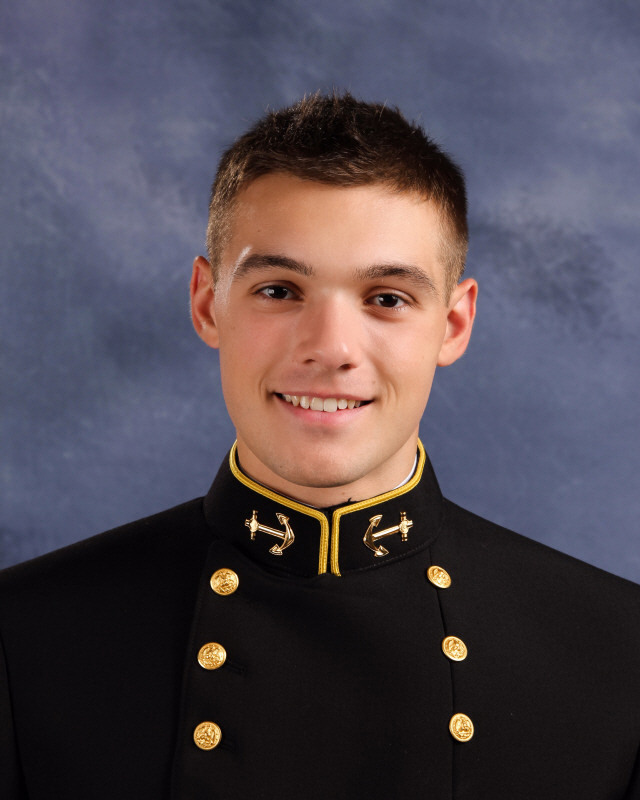
\includegraphics[width=1in,height=1.25in,clip,keepaspectratio]{\myroot/figures/M203876.jpg}}]{Ethan Marcello} is a midshipman at the United States Naval Academy majoring in Robotics and Control Engineering. Upon graduation, he hopes to service select as into either the pirate/privateer or blimp communities. 
\end{IEEEbiography}

\begin{IEEEbiography}[{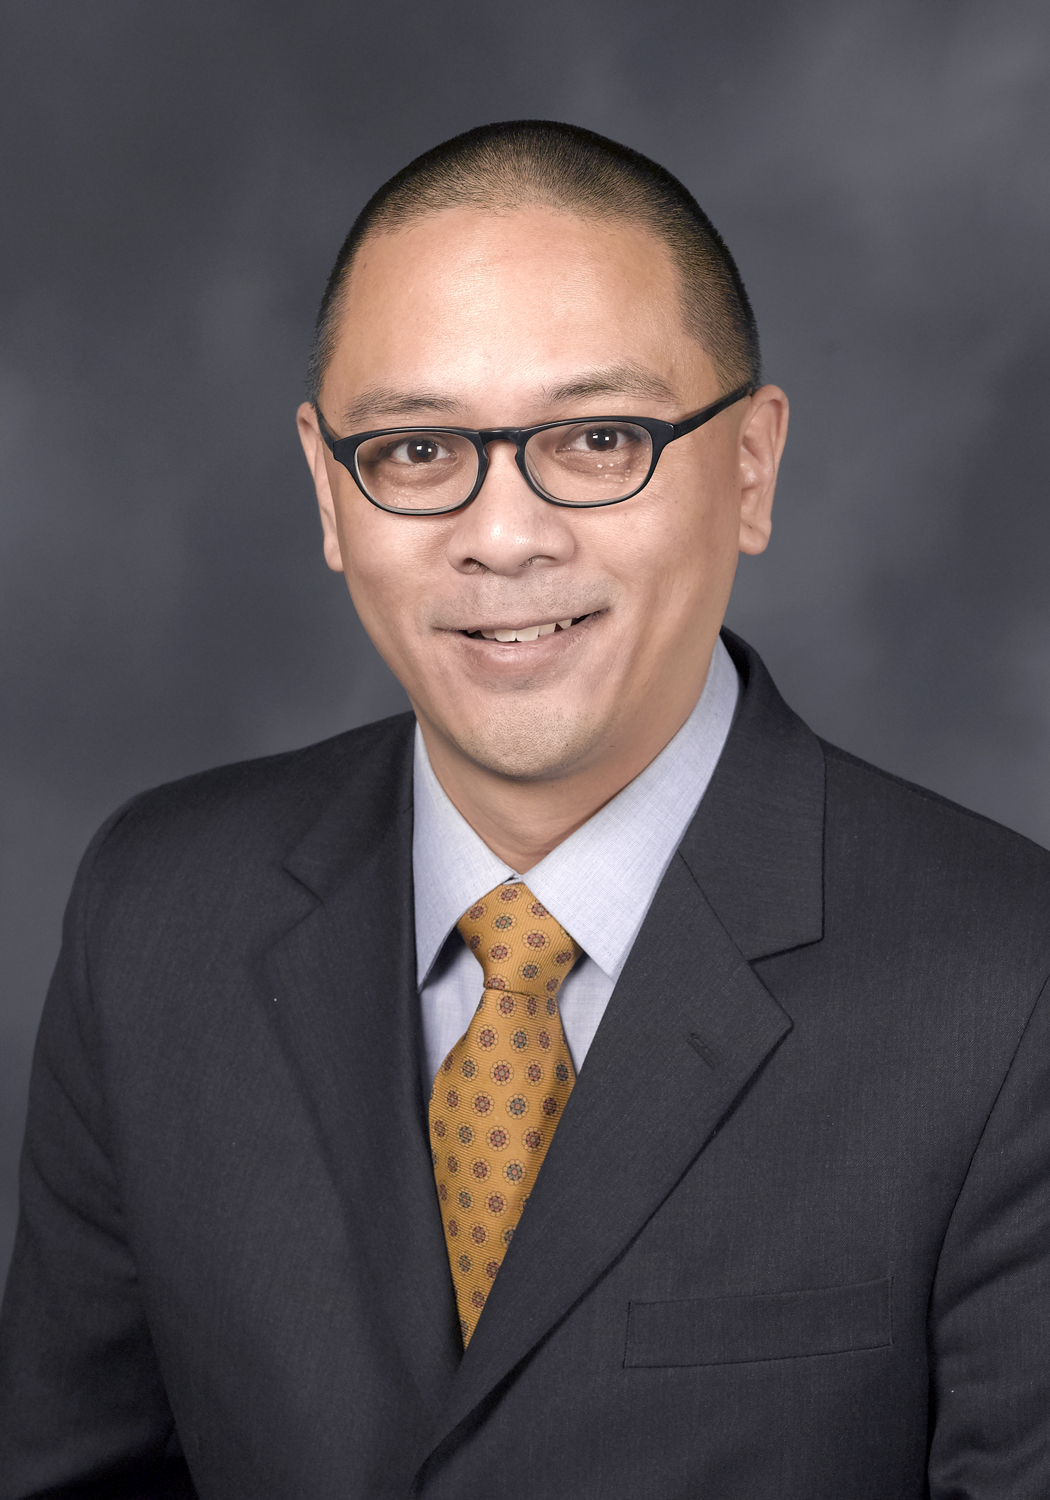
\includegraphics[width=1in,height=1.25in,clip,keepaspectratio]{\myroot/figures/evangelista_d_prof.jpg}}]{Dennis Evangelista} raises guide dog puppies. 
\end{IEEEbiography}

\end{document}